\section{Introduction}
\label{sec:intro}

Search-augmented language models answer from retrieved web pages, and those pages often disagree. The
disagreement can have very different causes. A question may be underspecified and admit several correct answers;
it may touch a contested topic on which reasonable sources differ; the answer may have changed over time, so some
pages are stale; or a page may simply be wrong. Each case calls for a different response: combine the answers,
present the viewpoints neutrally, prefer the most recent information, or ignore the unreliable source.
\citet{cattan2025dragged} formalised this as a five-way taxonomy, released \conflicts, a benchmark of 458 search
queries annotated by experts with their conflict type, and showed that giving a generator the gold type raises
the share of responses with the expected behaviour by about 24 points. Predicting the type is harder: the best LLM
they tested, Gemini~2.5 Flash, reached 65.3\% accuracy.

Conflict typing is a classification problem. It is made once per query, before the answer is written, and its
output is one of five labels. A classifier for it should therefore be fast enough to sit in front of every
search-augmented request, cheap enough to run on all of them, and calibrated enough that its uncertainty can be
acted on. A recent class of models, \emph{typed decision models}, is designed for this setting: they take
unstructured context and typed questions and return probabilities over the allowed answers in a single forward
pass, without generating text \citep{typesafe2026jev}. Since the first such model, several
providers have released their own, and one inference gateway now serves \ndm of them behind a common interface. Existing
evaluations cover classification, NLI and judging benchmarks, mostly for a single model
\citep{deusser2026jev,li2026specialized,duan2026general}, but none covers deciding why retrieved sources conflict,
a task that requires reading many documents at once and reasoning about their mutual relation rather than about
one text.

\begin{figure}[t]
\centering
% Overview of the study (Figure 1). Drawn in TikZ so that it uses the paper's fonts; \input by sections/method.tex.
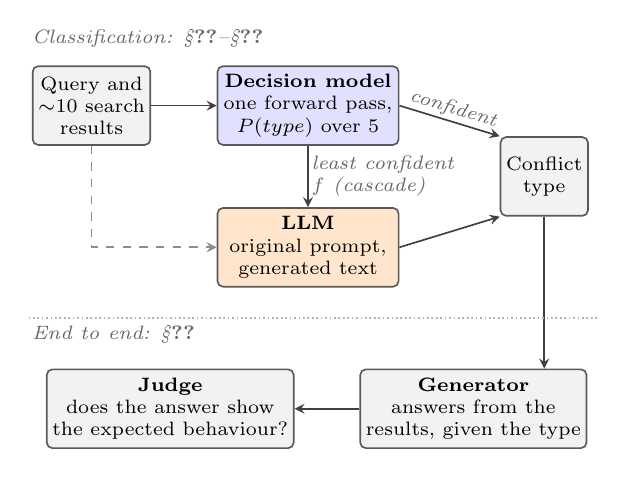
\begin{tikzpicture}[
  font=\scriptsize, >=stealth, line width=0.6pt,
  box/.style={draw=black!65, rounded corners=2pt, align=center, inner sep=2pt, minimum height=10mm},
  note/.style={font=\scriptsize\itshape, text=black!60, align=center, inner sep=1pt},
  arr/.style={->, draw=black!75}]
  % Classification.
  \node[box, fill=black!5, minimum width=14mm] (in) at (0, 0) {Query and\\$\sim$10 search\\results};
  \node[box, fill=blue!12, minimum width=23mm] (dm) at (2.75, 0) {\textbf{Decision model}\\one forward pass,\\$P(\text{type})$ over 5};
  \node[box, fill=orange!20, minimum width=23mm] (llm) at (2.75, -1.8) {\textbf{LLM}\\original prompt,\\generated text};
  \node[box, fill=black!5, minimum width=11mm] (type) at (5.75, -0.9) {Conflict\\type};
  \draw[arr] (in) -- (dm);
  \draw[arr] (dm.east) -- node[note, above, sloped] {confident} (type.north west);
  \draw[arr] (dm.south) -- node[note, right, align=left] {least confident\\$f$ (cascade)} (llm.north);
  \draw[arr] (llm.east) -- (type.south west);
  \draw[arr, dashed, draw=black!45] (in.south) |- (llm.west);
  % End to end.
  \node[box, fill=black!5, minimum width=27mm] (gen) at (4.85, -3.85) {\textbf{Generator}\\answers from the\\results, given the type};
  \node[box, fill=black!5, minimum width=27mm] (judge) at (1.0, -3.85) {\textbf{Judge}\\does the answer show\\the expected behaviour?};
  \draw[arr] (type.south) -- (type.south |- gen.north);
  \draw[arr] (gen) -- (judge);
  % Where each part is evaluated.
  \draw[black!30, densely dotted] (-0.8, -2.7) -- (6.45, -2.7);
  \node[note, anchor=north west] at (-0.8, 1.0) {Classification: \S\ref{sec:main}--\S\ref{sec:diagnostics}};
  \node[note, anchor=north west] at (-0.8, -2.75) {End to end: \S\ref{sec:endtoend}};
\end{tikzpicture}

\caption{Overview. A decision model types the conflict among a query's search results in one forward pass; in a
cascade, its least confident fraction $f$ of queries is typed by an LLM instead. End to end, a generator answers
given the predicted type, and a judge checks the answer against the expected behaviour of the gold type.}
\label{fig:overview}
\end{figure}

Can decision models, as a class, serve as this decision layer? And if only some can, what sets them apart? Our
study (Figure~\ref{fig:overview}) makes five contributions.

\paragraph{(1) A census of decision models on conflict typing.} We evaluate every decision model served by one
commercial gateway (\ndm models from \nproviders providers) on \conflicts under the original paper's protocol: the
same input representation, the same category definitions and examples taken verbatim from the paper's source, and
Gemini rerun on identical inputs so that every comparison is paired (\S\ref{sec:main}). \natpar of the \ndm
models match or exceed the paper's LLM at a fraction of its cost and latency; the current Gemini~3.8 Flash is
significantly more accurate than \nworsenow of them.

\paragraph{(2) A formulation study.} Decomposing the taxonomy into yes/no questions lowers accuracy for all \ndm
models, and a repair fitted on one model helps none, leaving the direct question as the reliable format
(\S\ref{sec:formulation}).

\paragraph{(3) Cost-quality cascades.} Decision models' confidence ranks their own errors, so sending their least
certain queries to an LLM is effective: with a quarter of the queries escalated to Gemini~3.8 Flash, \ncasctied of
the \ndm cascades are statistically tied with the LLM alone at \casctiedcostmin--\casctiedcostmax\% of its cost
(\S\ref{sec:cascade}).

\paragraph{(4) Pre-specified diagnostics.} We test whether decision models depend on publication dates,
are sensitive to source order, or miss a single false source among agreeing ones (\S\ref{sec:diagnostics}). Dates
play no measurable role, order sensitivity varies from model to model, and a planted false source shows in the
probabilities more than in the top answer.

\paragraph{(5) An end-to-end test.} Given to a generator, the types of \eentied of the \ndm decision models yield
answers that follow the expected behaviour as often as with the LLM's types, under both judges we specified
(\S\ref{sec:endtoend}).

Every setting and every later addition was fixed in writing before it was run (\S\ref{sec:setup}). We release the
code, prompts, splits and all model outputs\releasenote.
